\documentclass[11pt]{article}
\usepackage[top=2.8cm, bottom=2.8cm, left=1.5cm, right=1.5cm]{geometry}
\usepackage{hyperref}
\usepackage{algorithm2e}
\usepackage[numbers]{natbib}
\bibliographystyle{plainnat}
\usepackage{lscape}
\usepackage{gensymb}
\usepackage{appendix}
\usepackage[table]{xcolor}
\usepackage{pgfplots}
\usepackage{pgfplotstable}
\renewcommand{\familydefault}{\sfdefault}
\usepackage[font={color=darkgray,footnotesize, sf, it}]{caption}
\usepackage{amsmath}
\usepackage{helvet}
\usepackage{wrapfig}
\usepackage{multicol}
\usepackage[eulergreek]{sansmath}
\usepackage{listings}
\usepackage{setspace}
\usepackage{graphicx}
\usepackage{longtable}
\usepackage{minted}
\usepackage{relsize}
\linespread{1.2}
\lstset { %
    language=C++,
    backgroundcolor=\color{black!5}, % set backgroundcolor
    basicstyle=\ttfamily\footnotesize,% basic font setting
}
\usepackage{bchart}
\usepackage{booktabs}
\usepackage{xcolor}

\usepackage[english]{babel}
\usepackage[utf8]{inputenc}
\usepackage{fancyhdr}

\pagestyle{fancy}
\fancyhf{}
\rhead{cjd47 and ja663}
\lhead{CM30080: \textit{Computer Vision}}
\cfoot{\thepage} 
\renewcommand{\headrulewidth}{1pt}
\renewcommand{\footrulewidth}{1pt}

\lstdefinestyle{BashInputStyle}{
  language=bash,
  basicstyle=\footnotesize\ttfamily,
  numbers=left,
  numberstyle=\tiny,
  numbersep=3pt,
  frame=tb,
  columns=fullflexible,
  backgroundcolor=\color{cyan!20},
  linewidth=0.95\linewidth,
  xleftmargin=0.1\linewidth
}

\definecolor{skyblue}{RGB}{203,240,255}
\definecolor{forestgreen}{RGB}{0,96,50}
\definecolor{indigo}{RGB}{4,87,239}
\definecolor{darkindigo}{RGB}{1,40,112}
\definecolor{darkpurple}{RGB}{32,14,104}
\definecolor{apple}{RGB}{0,158,13}
\definecolor{bad}{RGB}{239,55,55}
\definecolor{badtoavg}{RGB}{247,128,98}
\definecolor{avg}{RGB}{255,218,117}
\definecolor{avgtogood}{RGB}{190,247,140}
\definecolor{good}{RGB}{102,226,102}

\date{}
\author{}
\setlength{\parindent}{0em}
\setlength{\parskip}{1em}
\setlength\parindent{0pt}

\usepackage{sectsty}
\sectionfont{\large}

\usepackage{tikz}
\usepackage{collcell}
\usetikzlibrary{shapes.geometric, arrows,calc}
\tikzstyle{startstop} = [rectangle, font=\small, rounded corners, minimum width=4cm, minimum height=0.8cm,text centered, text width=4.5cm, draw=black, fill=gray!50]
\tikzstyle{barrier} = [rectangle, font=\small, rounded corners, minimum width=4cm, minimum height=0.8cm,text centered, text width=4.5cm, draw=black, fill=red!50]
\tikzstyle{mainproc} = [rectangle, font=\small, minimum width=5cm, minimum height=0.8cm, text centered, text width=5cm, draw=black, fill=cyan!50]
\tikzstyle{threadproc} = [rectangle, font=\small, minimum width=4.5cm, minimum height=0.8cm, text centered, text width=4.5cm, draw=black, fill=orange!70]
\tikzstyle{decision} = [diamond, font=\small, align=center, minimum height=4ex, diamond, aspect=2, text width=14em, inner sep=-1pt, draw=black, fill=violet!50]
\tikzstyle{arrow} = [thick,->,>=stealth]
\tikzstyle{line} = [draw, -latex']

\makeatletter
\def\savepos#1{\leavevmode\pdfsavepos\write\@auxout{%
\gdef\string\save@#1{{\the\pdflastxpos sp }{\the\pdflastypos sp }}}}

\def\xx#1{\expandafter\expandafter\expandafter\@firstoftwo\csname save@#1\endcsname}
\def\yy#1{\expandafter\expandafter\expandafter\@secondoftwo\csname save@#1\endcsname}


\def\xsqrt#1{%
\sqrt{\vphantom{#1}}%
\ifx\save@L\@undefined
\else
\ifdim\yy{L}=\yy{R}%
\else
\rlap{$\overline{\vphantom{#1}\hskip\dimexpr\xx{b}-\xx{L}\relax}$}%
\fi
\fi
\savepos{L}#1\savepos{R}%
\ifx\save@L\@undefined
\else
\ifdim\yy{L}=\yy{R}%
\llap{$\overline{\hskip\dimexpr\xx{R}-\xx{L}\relax}$}%
\else
\llap{$\overline{\vphantom{#1}\hskip\dimexpr\xx{R}-\xx{a}\relax}$}%
\fi
\fi
}

\makeatother

\usepackage{titlesec}

\titlespacing\section{0pt}{11pt plus 4pt minus 2pt}{0pt plus 2pt minus 2pt}
\titlespacing\subsection{0pt}{11pt plus 4pt minus 2pt}{0pt plus 2pt minus 2pt}
\titlespacing\subsubsection{0pt}{11pt plus 4pt minus 2pt}{0pt plus 2pt minus 2pt}

\title{{\color{indigo}\textbf{CM30080: Computer Vision}}\\\small \textbf{Filtering, Object Recognition \& Features\\April 2019}\vspace{-15ex}}
\SetKwInOut{Parameter}{parameter}

\begin{document}
\normalsize
\pgfplotsset{compat=1.16}

\setlength{\multicolsep}{19pt}
\begin{multicols}{2}

{\color{indigo}
\section{Image convolution}}
Firstly, the kernel is rotated 180\textdegree \ and the image is padded with zeros on all sides before sliding the kernel horizontally across the image and calculating the sum of the element-wise product of the flipped kernel and image. This is expressed as: $(I*f)(x,y)=\sum_{k}\sum_{l}I(k,l)f(x-k,y-l)$. Results of this function were shown to match the output of MATLAB's built-in \texttt{conv2} function (\texttt{\hyperlink{convolutionTestScript.m}{convolutionTestScript.m}}). A range of images from the training dataset were convolved with a range of kernels using blurs of different kernel sizes and $\sigma$ values, and edge detectors in different directions. See \texttt{\hyperlink{convolution.m}{convolution.m}} for details. A larger $\sigma$ in a Gaussian kernel produced a smoother blur. Applying Sobel high pass filters displayed edges. Combining filters allowed effects such as sharpening due to the distribution property of $*$.

{\color{indigo}
\section{Intensity-based template matching}}
Initially, a Gaussian Pyramid (GP) was created by applying a Gaussian filter $G(x,y,\sigma)$ to each training image class at a variety of rotations before sub-sampling by a factor of 2 across a series of octaves, to generate templates. Each resulting blurred image can be expressed as $L(x,y,\sigma)=G(x,y,\sigma)*I(x,y)$. Intensity-based matching (IBM) necessitated computing the correlation between templates and test images. The template yielding the maximum correlation across the test image was determined for each training image class before a non-maxima suppression (NMS) strategy was applied to ensure detection occurred at sensible correlation values. NMS involved suppressing classes of templates with a bounding box overlapping that of the template with the maximum correlation score.

A computationally-expensive approach slides the patch across the entire test image and computes the correlation at each point $(x,y)$ using the formula: $cor(x,y)=\sum_{i,j}T(i,j)I(x+i,y+j)$. A more efficient approach involves using the Fast Fourier Transform (FFT) to transform the image signal into the frequency domain for faster processing. Multiplication in the Fourier domain is equivalent to convolution in the real domain ($f*g=\mathcal{F}^{-1}\{ \mathcal{F}\{f\} \cdot \mathcal{F}\{g\} \}$), so the correlation result can also be efficiently determined by taking the inverse FT of the product of the FT of the image and template. MATLAB's \texttt{normxcorr2} function was used as it utilises this property. This was applied separately to each RGB channel before averaging the result. See \texttt{\hyperlink{runIntensityMatching.m}{runIntensityMatching.m}} for details.

Table 1 shows the optimum results of running IBM detection on a test image with NMS applied and a $5\times5$ Gaussian kernel with $\sigma=1,2,4,8$ across $5$ octaves (chosen as the smallest image across all test images was a factor of $2^{-4}$ of the original size). Each octave's image had $12$ rotations applied before subsampling which was a pragmatic compromise as the average runtime with this number was already $1039.1$s.  IBM (Fig 1) finds difficulty where icons in test images were directly in-between multiples of the rotation or size of the templates in the GP as pixels do not line up as optimally. IBM's runtime complexity is $O(ijk nm\log nm)$ for $i$ rotations, $j$ octaves, $k$ training images where $n$ is the image height and $m$ is the image width. Memory complexity is therefore $O(ijknm)$ to store all images in the GP. IBM generated templates invariant to rotation and scale, but not to illumination. It is also heavily dependent on the quantity of unique rotations and scales used in the pyramid. As such, Task 3 used SIFT to generate \textit{features} for more robust template matching.

\setlength\abovedisplayskip{0pt}
\setlength\belowdisplayskip{0pt}
\begin{table}[H]
\begin{center}
\resizebox{0.8\linewidth}{!}{%
\begin{tabular}{|c|c|c|c|c|c|c|}
\hline
\textbf{TP Rate} & \textbf{FP Rate} & \textbf{ACC} & \textbf{Avg Runtime}\\
\hline
56.7\% & 8.9\% & 87.0\% & 1039.1s\\
\hline
\end{tabular}}
\label{tbl:t2results}\caption{TP, FP, ACC Results and Runtime for Task 2.}
\end{center}
\end{table}
\vspace*{-\baselineskip}
\normalsize

\setlength\abovedisplayskip{0pt}
\setlength\belowdisplayskip{0pt}
\begin{figure}[H]
\centering
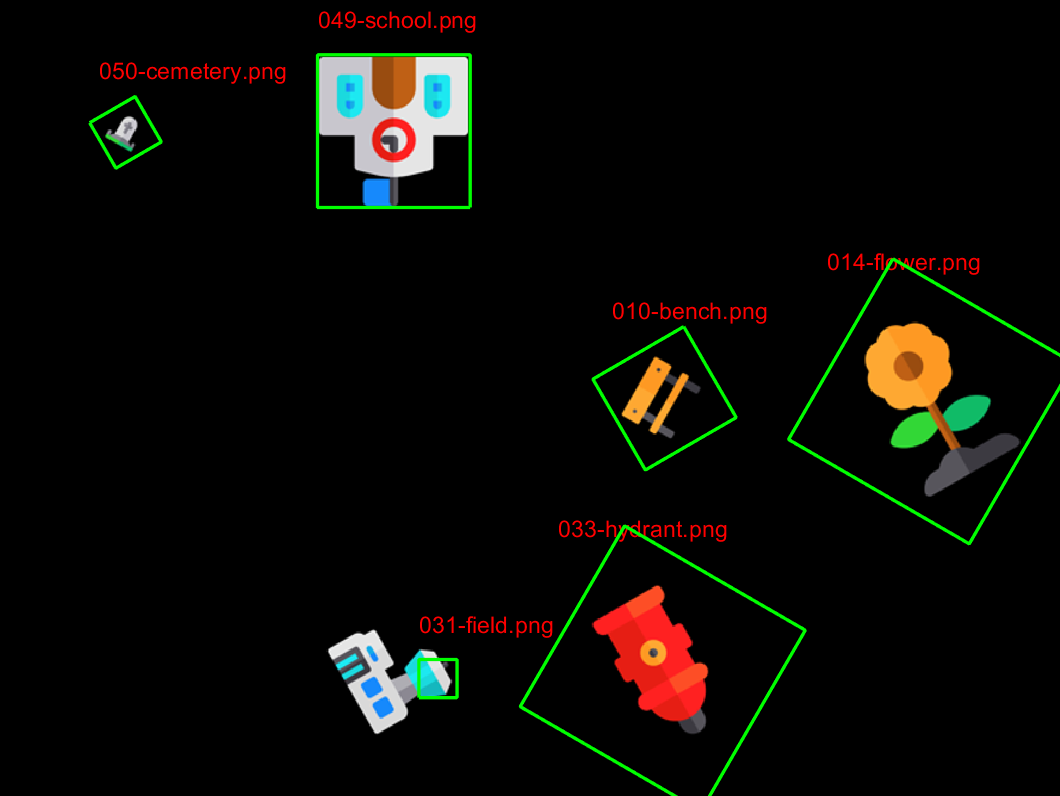
\includegraphics[width=0.65\linewidth]{img/IBM.png} 
\caption{IBM detection on a test image.}\label{fig:IBM}
\end{figure}
\vspace*{-\baselineskip}

{\color{indigo}
\section{Feature-based template matching (SIFT)}}
Lowe's SIFT algorithm \cite{lowe1999,lowe2004} was used to identify correspondences between features of the training set and each test image in order to identify the classes of objects present in each test image.  Keypoint localisation involved creating a Difference of Gaussian (DoG) pyramid of $4$ octaves (levels), with a set of $4$ blurs applied, varying $\sigma$ at each octave to form an approximation for the Laplacian of Gaussians (LoG) (i.e. $\nabla^2g_{\sigma} \approx (g_{\sigma_1}-g_{\sigma_2})*I$). This allowed for extrema in the $(x,y,\sigma)$ space to be identified as keypoints by comparing a point $(x,y)$ in the current DoG against all its neighbours in a $3\times3\times3$ patch across the current, previous and next DoGs. All points $(x,y,\sigma)$ identified as unique extrema were filtered by discarding points in the DoG with a contrast below a threshold ($<0.12$). Then, the Hessian matrix $\mathbf{H}$ was approximated using the image gradient at each keypoint to discard edges (points in the DoG with $r>10$). Corner values were favoured as they hold more valuable information (Fig 2). 

\setlength\abovedisplayskip{0pt}
\setlength\belowdisplayskip{0pt}
\setlength\multicolsep{0pt}
\begin{multicols}{2}
\begin{equation*}
\mathbf{H}=\begin{bmatrix}
      D_{xx} & D_{xy} \\
      D_{xy} & D_{yy} \\
     \end{bmatrix}
\end{equation*}\break
\begin{equation*}
\dfrac{Tr(\mathbf{H})^2}{Det(\mathbf{H})}=\dfrac{(r+1)^2}{r}
\end{equation*}
\end{multicols}

A rotation orientation was then calculated for each keypoint $L(x,y,\sigma)$ equal to the dominant orientation $\theta(x,y)$ of the gradient $m(x,y)$, based on a historgram of 36 bins in which the orientations of values in a surrounding $15\times15$ window were stored. Values were weighted by the magnitude of the gradient at each keypoint and a Gaussian-weighted circular window with a scale of $1.5\sigma$. This characterised keypoints as $(x,y,\sigma,\theta)$ to provide rotation invariance by rotating keypoints by this value. Histogram peaks $>80\%$ of the highest peak were converted into new keypoints $(x,y,\sigma,\theta^{'})$. Finally, a SIFT feature (128 dimensional vector) was generated for each keypoint using a $16\times16$ window split into $4\times4$ cells with each cell being represented by an 8 bin histogram of gradient magnitude and orientation (Fig 3). Each bin entry was weighted by a value $w=1-d$ where $d$ represents the distance of the value from the central value, normalised by the width of the bin. The window also had a Gaussian weighting applied. The resulting 16 histograms formed the SIFT descriptor. After features are generated for training and test images, a suitable correspondence between two feature vectors $\phi^{(1)}, \phi^{(2)}$ was found by an $SSD$ matching function. This was calculated between all the features in each training image class against all the features in the test image. Matches were refined by filtering with an empirically-tested $SSD$ threshold of $0.3$ and nearest-neighbour ratio (NNR) to discard weak matches (where $R>0.8$).

\setlength\multicolsep{0pt}
\setlength\abovedisplayskip{0pt}
\setlength\belowdisplayskip{0pt}
\begin{multicols}{2}
\begin{equation*}
SSD=\sum_{i=1}^{128}(\phi_i^{(1)}-\phi_i^{(2)})^2
\end{equation*}\break
\begin{equation*}
R=\dfrac{SSD(\phi^{(1)},\phi^{(2)})}{SSD(\phi^{(1)},\phi^{'(2)})}
\end{equation*}
\end{multicols}

For SIFT object recognition in a given test image (Fig 4), the summation of the $SSD$s of all feature matches (after thresholding and NNR) was calculated for each training image class. This value was normalised by dividing by the number of total matches detected between the training image in question and the test image. The training image class yielding the minimum normalised $SSD$ summation was selected as the most suitable class. Matches containing features in the test image and the most suitable training image class were removed from the list of all matches before the process was repeated for each of the remaining objects in the test image. See \texttt{\hyperlink{runSIFT.m}{runSIFT.m}} for details.

\setlength\abovedisplayskip{0pt}
\setlength\belowdisplayskip{0pt}
\begin{figure}[H]
\centering
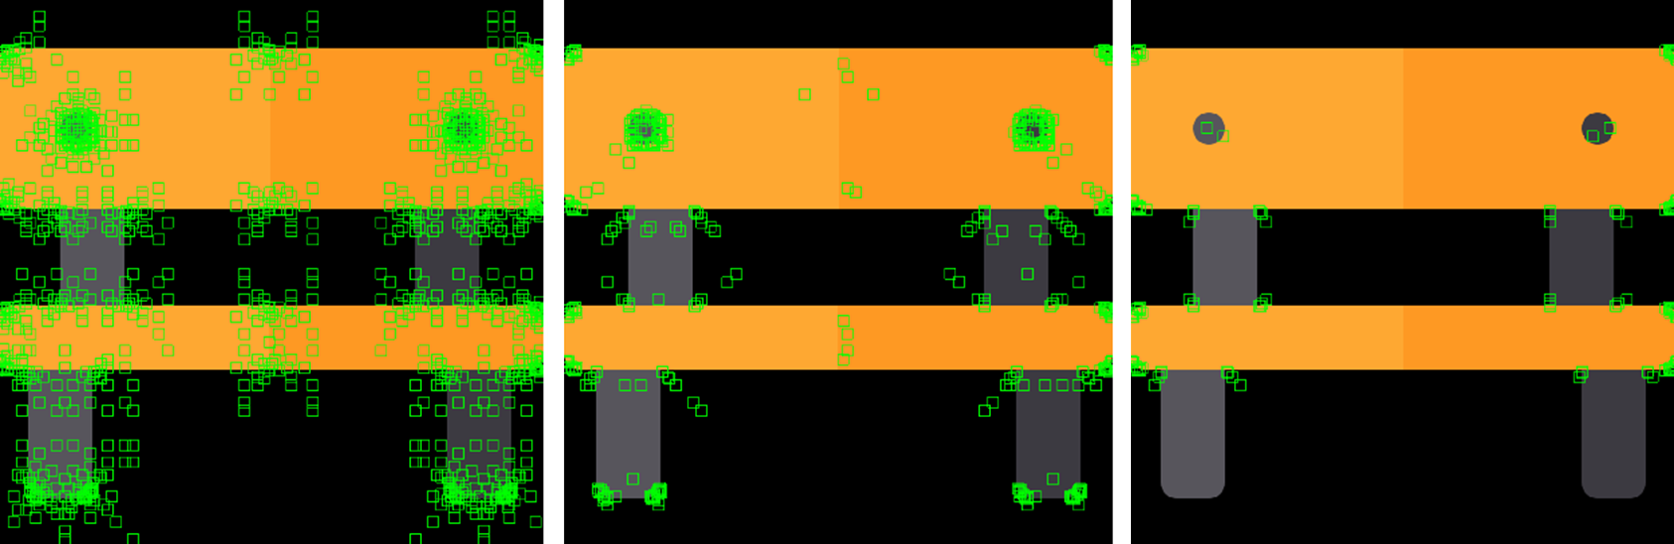
\includegraphics[width=0.9\linewidth]{img/EDGECONTRAST.png} 
\caption{All keypoints (left), post-edge removal (mid) and post-contrast thresholding and edge removal (right).}\label{fig:EDGECONTRAST}
\end{figure}
\vspace*{-\baselineskip}

\setlength\abovedisplayskip{0pt}
\setlength\belowdisplayskip{0pt}
\begin{figure}[H]
\centering
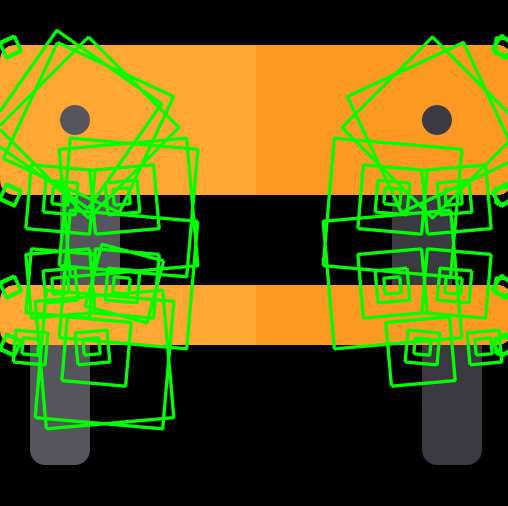
\includegraphics[width=0.35\linewidth]{img/BenchSIFTFeatures.png} 
\caption{SIFT features extracted from a training image.}\label{fig:BenchSIFTFeatures}
\end{figure}
\vspace*{-\baselineskip}

\setlength\abovedisplayskip{0pt}
\setlength\belowdisplayskip{0pt}
\begin{figure}[H]
\centering
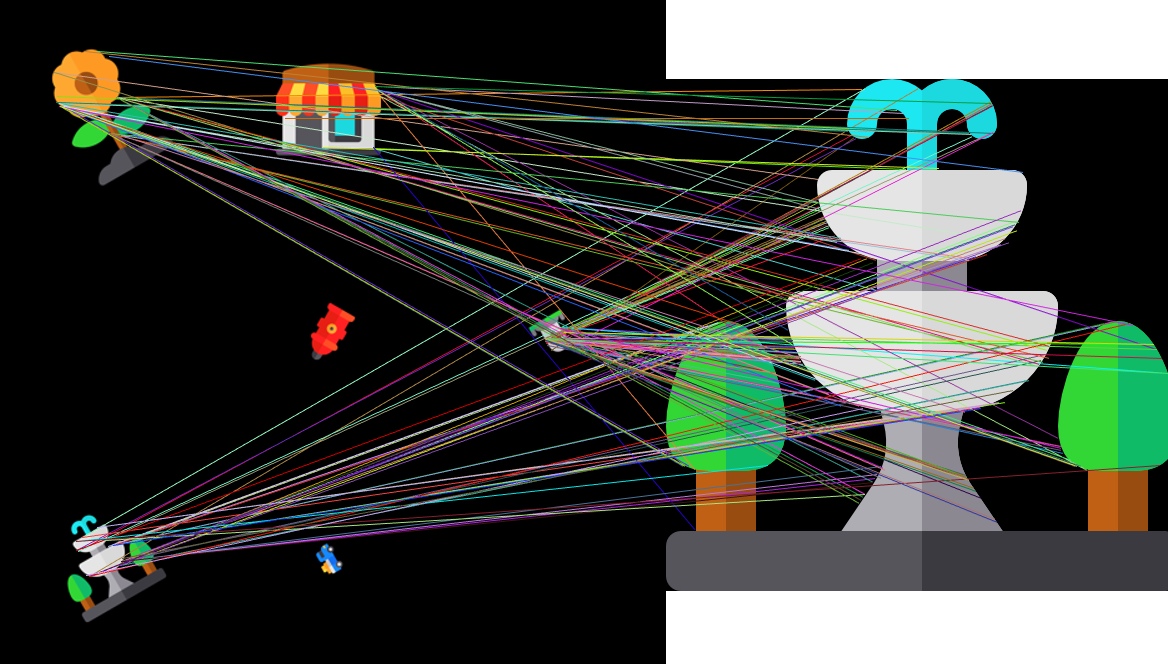
\includegraphics[width=0.65\linewidth]{img/SIFTMATCHES.png} 
\caption{SIFT matching between a test (left) and training (right) image.}\label{fig:SIFTMATCHES}
\end{figure}
\vspace*{-\baselineskip}

Table 2 shows the optimum results of running SIFT detection on a test image. This was produced using a $5\times5$ Gaussian kernel with $\sigma=0.4$ initially and increasing by a factor of $2.5$ per octave across $5$ octaves with the $SSD$ threshold and $R$ values described previously. This parameter choice was justified by empirical results (Fig 5), which was inspired by the empirical graphs of Lowe \citep{lowe2004}. The implementation of edge detection was not optimal, which meant the SIFT detector found difficulty distinguishing icons with similar edge features such as the Bank and Courthouse. To improve this implementation, subpixel localisation using the Taylor series would increase accuracy of keypoints, and Hough Transform voting could assist with cluster identification \citep{lowe2004}. SIFT ran in real-time and could perform detection 10 times faster ($\approx 97.3$s) than IBM. SIFT's runtime complexity was $O(n_{1}n_{2} + m)$ for $n_1$ training features, $n_2$ test features and $m$ matches as the complexity of $SSD$ operations is constant due to the fixed feature vector size and the number of matches is what determines the remaining processing. In other words, SIFT detection's runtime complexity is independent of image size (unlike IBM) and dependent on the number of features and matches between training and test images instead. Memory complexity is dominated by the number of feature vectors and is therefore $O(n_{1}+n_{2})$, making SIFT more scalable than IBM when larger input images are considered.

\setlength\abovedisplayskip{0pt}
\setlength\belowdisplayskip{0pt}
\begin{figure}[H]
\centering
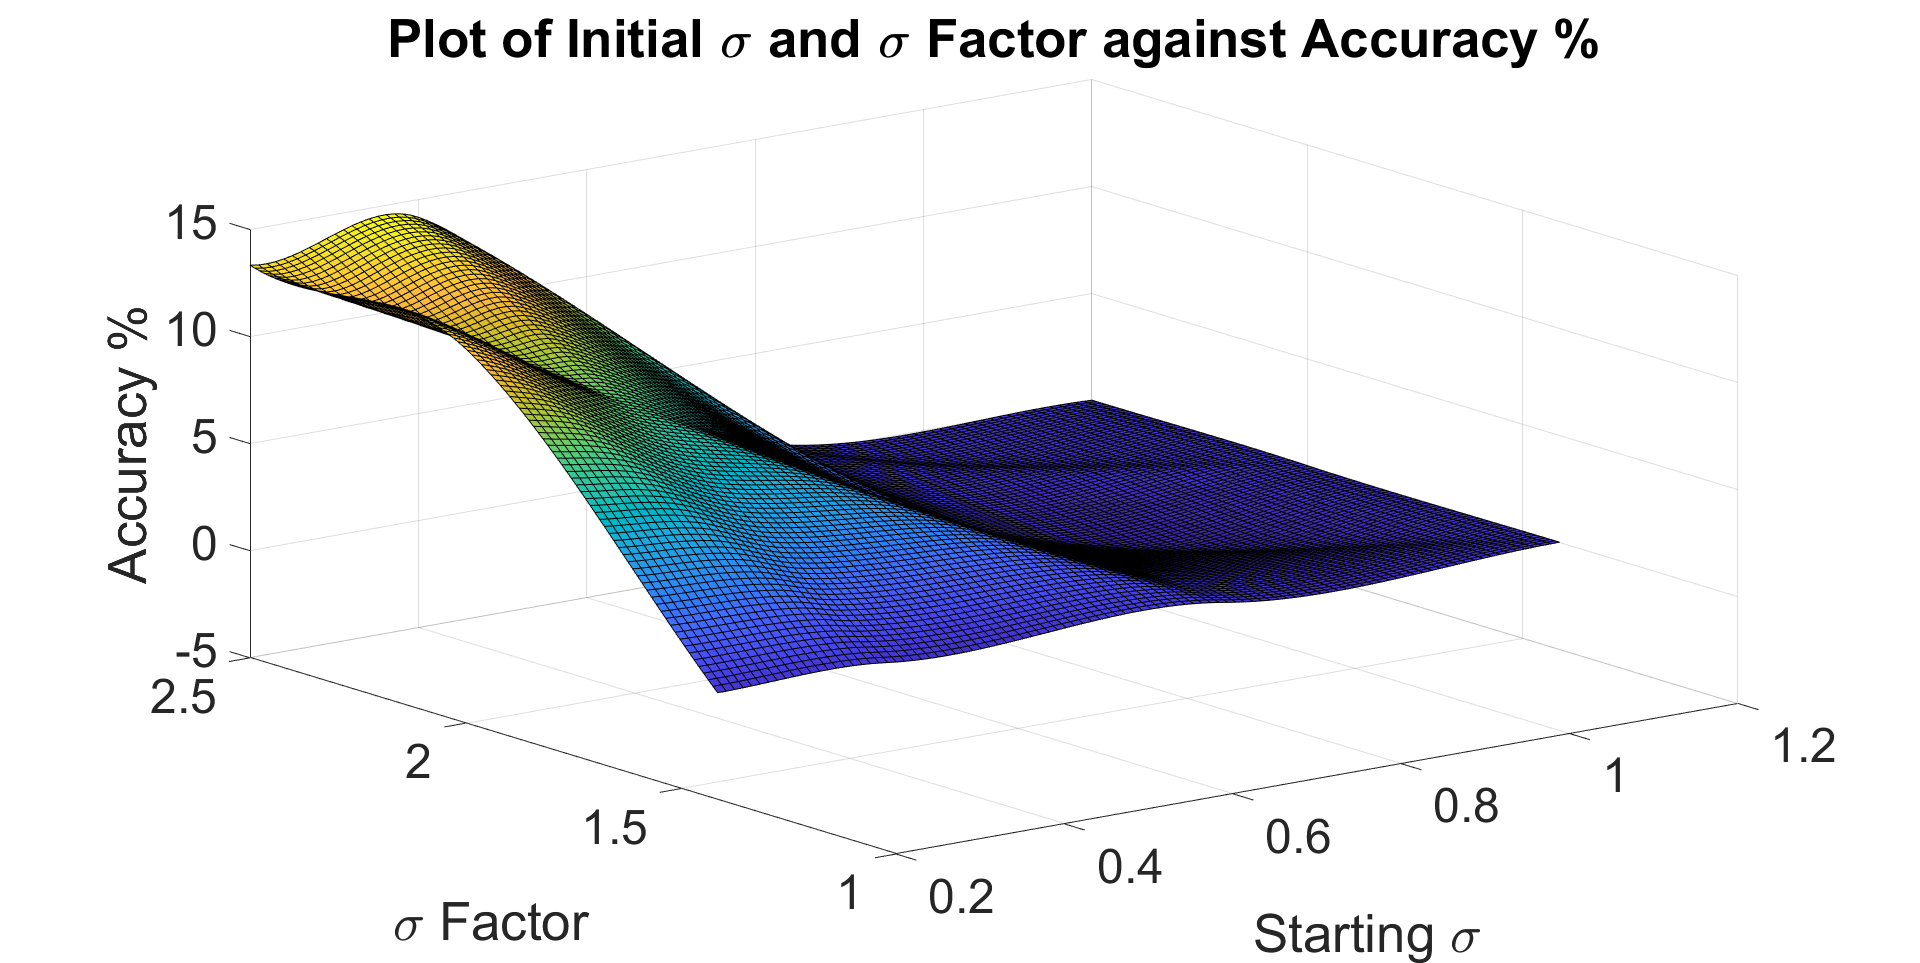
\includegraphics[width=\linewidth]{img/sift-plot.png} 
\label{fig:sift-plot}\caption{Initial $\sigma$ and $\sigma$ factor against accuracy \%.}
\end{figure}
\vspace*{-\baselineskip}

\setlength\abovedisplayskip{0pt}
\setlength\belowdisplayskip{0pt}
\begin{table}[H]
\begin{center}
\resizebox{0.4\linewidth}{!}{%
\begin{tabular}{|c|c|}
\hline
\textbf{ACC} & \textbf{Avg Runtime}\\
\hline
14.2\% & 97.3s\\
\hline
\end{tabular}}
\label{tbl:t3results}\caption{ACC Results and Runtime for Task 3.}
\end{center}
\end{table}
\vspace*{-\baselineskip}

\scriptsize
\bibliography{Bibliography}
\normalsize
\end{multicols}

\newpage
{\color{indigo}
\section*{Contributions}}
\begin{table}[H]
\begin{tabular}{|c|c|p{8cm}|c|}
\hline
\textbf{Name} & \textbf{Username} & \textbf{Contribution} & \textbf{Contribution \%}\\
\hline
Christopher Davies & cjd47 & Code and report & 50\%\\
\hline
James Armitstead & ja663 & Code and report & 50\%\\
\hline
\end{tabular}
\end{table}

\newpage
\begin{appendices}

{\color{indigo}
\section{Code}
\label{apdx:code}}
\subsection*{calcGradientAngle.m} \label{sec:calcGradientAngle.m}
\inputminted[breaklines=true,breakanywhere=true,fontsize=\small]{matlab}{../src/calcGradientAngle.m}

\subsection*{\hypertarget{convolution.m}{convolution.m}}
\label{sec:convolution.m}
\inputminted[breaklines=true,breakanywhere=true,fontsize=\small]{matlab}{../src/convolution.m}

\subsection*{\hypertarget{doesIntersect.m}{doesIntersect.m}}
\label{sec:doesIntersect.m}
\inputminted[breaklines=true,breakanywhere=true,fontsize=\small]{matlab}{../src/doesIntersect.m}

\subsection*{drawFeatureMatches.m}
\label{sec:drawFeatureMatches.m}
\inputminted[breaklines=true,breakanywhere=true,fontsize=\small]{matlab}{../src/drawFeatureMatches.m}

\subsection*{drawIntensityMatches.m}
\label{sec:drawIntensityMatches.m}
\inputminted[breaklines=true,breakanywhere=true,fontsize=\small]{matlab}{../src/drawIntensityMatches.m}

\subsection*{drawSIFTDescriptors.m}
\label{sec:drawSIFTDescriptors.m}
\inputminted[breaklines=true,breakanywhere=true,fontsize=\small]{matlab}{../src/drawSIFTDescriptors.m}

\subsection*{generateMatches.m}
\label{sec:generateMatches.m}
\inputminted[breaklines=true,breakanywhere=true,fontsize=\small]{matlab}{../src/generateMatches.m}

\subsection*{generateResults.m}
\label{sec:generateResults.m}
\inputminted[breaklines=true,breakanywhere=true,fontsize=\small]{matlab}{../src/generateResults.m}

\subsection*{generateScores.m}
\label{sec:generateScores.m}
\inputminted[breaklines=true,breakanywhere=true,fontsize=\small]{matlab}{../src/generateScores.m}

\subsection*{generateTemplates.m}
\label{sec:generateTemplates.m}
\inputminted[breaklines=true,breakanywhere=true,fontsize=\small]{matlab}{../src/generateTemplates.m}

\subsection*{getAllFeatureDescriptors.m}
\label{sec:getAllFeatureDescriptors.m}
\inputminted[breaklines=true,breakanywhere=true,fontsize=\small]{matlab}{../src/getAllFeatureDescriptors.m}

\subsection*{getAllMaxCorrelations.m}
\label{sec:getAllMaxCorrelations.m}
\inputminted[breaklines=true,breakanywhere=true,fontsize=\small]{matlab}{../src/getAllMaxCorrelations.m}

\subsection*{getBestMatches.m}
\label{sec:getBestMatches.m}
\inputminted[breaklines=true,breakanywhere=true,fontsize=\small]{matlab}{../src/getBestMatches.m}

\subsection*{getDoGsAndBlurs.m}
\label{sec:getDoGsAndBlurs.m}
\inputminted[breaklines=true,breakanywhere=true,fontsize=\small]{matlab}{../src/getDoGsAndBlurs.m}

\subsection*{getExtrema.m}
\label{sec:getExtrema.m}
\inputminted[breaklines=true,breakanywhere=true,fontsize=\small]{matlab}{../src/getExtrema.m}

\subsection*{getFeatureDescriptor.m}
\label{sec:getFeatureDescriptor.m}
\inputminted[breaklines=true,breakanywhere=true,fontsize=\small]{matlab}{../src/getFeatureDescriptor.m}

\subsection*{getImagePaths.m}
\label{sec:getImagePaths.m}
\inputminted[breaklines=true,breakanywhere=true,fontsize=\small]{matlab}{../src/getImagePaths.m}

\subsection*{getRotationOrientation.m}
\label{sec:getRotationOrientation.m}
\inputminted[breaklines=true,breakanywhere=true,fontsize=\small]{matlab}{../src/getRotationOrientation.m}

\subsection*{isCorner.m}
\label{sec:isCorner.m}
\inputminted[breaklines=true,breakanywhere=true,fontsize=\small]{matlab}{../src/isCorner.m}

\subsection*{maxCorrelation.m} 
\label{sec:maxCorrelation.m}
\inputminted[breaklines=true,breakanywhere=true,fontsize=\small]{matlab}{../src/maxCorrelation.m}

\subsection*{minMaxCount.m} 
\label{sec:minMaxCount.m}
\inputminted[breaklines=true,breakanywhere=true,fontsize=\small]{matlab}{../src/minMaxCount.m}

\subsection*{plotSIFTAccuracy.m}
\label{sec:plotSIFTAccuracy.m}
\inputminted[breaklines=true,breakanywhere=true,fontsize=\small]{matlab}{../src/plotSIFTAccuracy.m}

\subsection*{reduceScores.m}
\label{sec:reduceScores.m}
\inputminted[breaklines=true,breakanywhere=true,fontsize=\small]{matlab}{../src/reduceScores.m}

\subsection*{resizeImage.m}
\label{sec:resizeImage.m}
\inputminted[breaklines=true,breakanywhere=true,fontsize=\small]{matlab}{../src/resizeImage.m}

\subsection*{\hypertarget{runIntensityMatching.m}{runIntensityMatching.m}}
\label{sec:runIntensityMatching.m}
\inputminted[breaklines=true,breakanywhere=true,fontsize=\small]{matlab}{../src/runIntensityMatching.m}

\subsection*{\hypertarget{runSIFT.m}{runSIFT.m}}
\label{sec:runSIFT.m}
\inputminted[breaklines=true,breakanywhere=true,fontsize=\small]{matlab}{../src/runSIFT.m}

{\color{indigo}
\section{Test Scripts}
\label{apdx:test-scripts}}
\subsection*{\hypertarget{convolutionTestScript.m}{convolutionTestScript.m}}
\label{sec:convolutionTestScript.m}
\inputminted[breaklines=true,breakanywhere=true,fontsize=\small]{matlab}{../src/convolutionTestScript.m}

\end{appendices}
\end{document}